%!TEX root = 02-np-SL.tex

\begin{document}

\title[NP-completeness]
{NP-completeness}

\begin{frame}
	\titlepage
\end{frame}

\lecturenotes{\maketitle}

\begin{frame}
	\slides{\frametitle{Outline}}
	\tableofcontents
\end{frame}


\section{Overview}

\begin{frame}
	\slides{\frametitle{Polynomial time}}
	\begin{block}{Polynomial-time algorithm}
		Polynomial-time algorithm:\\
		There exists a constant $c\in \mathbb{N}$ such that the algorithm has (worst-case) running-time $O(n^c)$, where $n$ is the size of the input.
	\end{block}

	\pause
	\begin{block}{Example}
		Polynomial: $n$; ~$n^2 \log_2 n$; ~$n^3$; ~$n^{20}$\\
		Super-polynomial: $n^{\log_2 n}$; ~$2^{\sqrt{n}}$; ~$1.001^n$; ~$2^n$; ~$n!$
	\end{block}

\end{frame}


\begin{frame}
	\slides{\frametitle{Tractable problems}}

	\begin{block}{Central Question}
		Which computational problems have polynomial-time algorithms?
	\end{block}

\end{frame}

\begin{frame}{Million-dollar question}

	Intriguing class of problems: \NP-complete problems.

	\begin{block}{NP-complete problems}
		It is unknown whether \NP-complete problems have polynomial-time algorithms.
		\begin{itemize}
			\item A polynomial-time algorithm for one \NP-complete problem would imply polynomial-time algorithms for all problems in \NP.
		\end{itemize}
	\end{block}

	Gerhard Woeginger's \P\ vs \NP\ page: \url{http://www.win.tue.nl/~gwoegi/P-versus-NP.htm}

\end{frame}


\begin{frame}{Polynomial vs. NP-complete}

	\begin{columns}
		\begin{column}[t]{.48\textwidth}
			{\slides{\color{Green}\rule{\linewidth}{4pt}\\
					\hspace{1.8cm}} Polynomial\\
				\slides{\rule{\linewidth}{4pt}}\\}

			\begin{itemize}
				\item \textsc{Shortest Path}: Given a graph $G$, two vertices $a$ and $b$ of $G$, and an integer $k$, does $G$ have a simple $a$--$b$-path of length at most $k$?
				\item \textsc{Euler Tour}: Given a graph $G$, does $G$ have a cycle that traverses each edge of $G$ exactly once?
				\item \textsc{2-CNF SAT}: Given a propositional formula $F$ in 2-CNF, is $F$ satisfiable?\\\emph{A \alert{$k$-CNF formula} is a conjunction (AND) of clauses, and each clause is a disjunction (OR) of at most $k$ literals, which are negated or unnegated Boolean variables.}
			\end{itemize}
		\end{column}%
		\hfill%
		\begin{column}[t]{.48\textwidth}
			{\slides{\color{red}\rule{\linewidth}{4pt}\\
					\hspace{1.8cm} \NP-complete \\
					\rule{\linewidth}{4pt}}\\}

			\lecturenotes{NP-complete}

			\begin{itemize}
				\item \textsc{Longest Path}: Given a graph $G$ and an integer $k$, does $G$ have a simple path of length at least $k$?
				\item \textsc{Hamiltonian Cycle}: Given a graph $G$, does $G$ have a simple cycle that visits each vertex of $G$?
				\item \textsc{3-CNF SAT}: Given a propositional formula $F$ in 3-CNF, is $F$ satisfiable?\\\emph{ Example: $(x \vee \neg y \vee z) \wedge (\neg x \vee z) \wedge (\neg y \vee \neg z)$.}
			\end{itemize}
		\end{column}%
	\end{columns}

\end{frame}


\begin{frame}{Overview}
	What's next?
	\begin{itemize}
		\item Formally define \P, \NP, and \NP-complete (\NPC)
		\item (New) skill: show that a problem is \NP-complete
		      %\item Briefly: what to do when confronted with an \NP-complete problem?
	\end{itemize}
\end{frame}


\section{Turing Machines, P, and NP}

\begin{frame}{Decision problems and Encodings}
	\pbDefNoPara{$<$Name of Decision Problem$>$}{$<$What constitutes an instance$>$}{$<$\alert{Yes/No} question$>$}

	\pause
	We want to know which decision problems can be solved in polynomial time -- polynomial in the \alert{size of the input} $n$.
	\begin{itemize}
		\item Assume a ``reasonable'' encoding of the input
		\item Many encodings are polynomial-time equivalent; i.e., one encoding can be computed from another in polynomial time.
		\item Important exception: unary versus binary encoding of integers.
		      \begin{itemize}
			      \item An integer $x$ takes $\lceil \log_2 x \rceil$ bits in binary and $x = 2^{\log_2 x}$ bits in unary.
		      \end{itemize}
	\end{itemize}
\end{frame}


\begin{frame}{Formal-language framework}
	We can view decision problems as languages.
	\begin{itemize}
		\item Alphabet $\Sigma$: finite set of symbols. W.l.o.g., $\Sigma=\{0,1\}$
		\item Language $L$ over $\Sigma$: set of strings made with symbols from $\Sigma$: $L \subseteq \Sigma^*$
		\item Fix an encoding of instances of a decision problem $\Pi$ into $\Sigma$
		\item Define the language $L_{\Pi} \subseteq \Sigma^*$ such that
	\end{itemize}
	\begin{align*}
		x\in L_{\Pi} \Leftrightarrow x \text{ is a Yes-instance for } \Pi
	\end{align*}
\end{frame}


\begin{frame}{Non-deterministic Turing Machine (NTM)}

	\begin{columns}
		\begin{column}[t]{.50\textwidth}
			\begin{itemize}
				\item \alert{input word} $x\in \Sigma^*$ placed on an \alert{infinite tape} (memory)
				\item read-write head initially placed on the first symbol of $x$
				\item computation step: if the machine is in state $s$ and reads $a$, it can move into state $s'$, writing $b$, and moving the head into direction $D \in \{L,R\}$ if $((s,a),(s',b,D)) \in \delta$.
			\end{itemize}
			\centering
			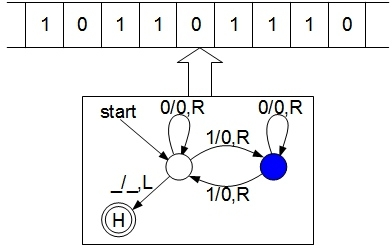
\includegraphics[scale=0.3]{./img/tm.jpg}
			% tm.pdf: 842x595 pixel, 72dpi, 29.70x20.99 cm, bb=0 0 842 595
		\end{column}
		\begin{column}[t]{.50\textwidth}
			\begin{itemize}
				\item $Q$: finite, non-empty set of states
				\item $\Gamma$: finite, non-empty set of tape symbols
				\item $\_\in \Gamma$: blank symbol (the only symbol allowed to occur on the tape infinitely often)
				\item $\Sigma\subseteq\Gamma\setminus\{b\}$: set of input symbols
				\item $q_0 \in Q$: start state
				\item $A \subseteq Q$: set of accepting (final) states
				\item $\delta \subseteq (Q \setminus A \times \Gamma) \times (Q \times \Gamma \times \{L,R\})$: transition relation, where $L$ stands for a move to the left and $R$ for a move to the right.
			\end{itemize}
		\end{column}
	\end{columns}

\end{frame}

\begin{frame}{Accepted Language}
	\begin{definition}
		A NTM \alert{accepts} a word $x\in \Sigma^*$ if there exists a sequence of computation steps starting in the start state and ending in an accept state.
	\end{definition}
	\begin{definition}
		The language \alert{accepted} by an NTM is the set of words it accepts.
	\end{definition}
\end{frame}

\lecturenotes{
	\begin{frame}{Video}
		\begin{center}
			The LEGO Turing Machine\\
			\url{https://www.youtube.com/watch?v=cYw2ewoO6c4}
		\end{center}
	\end{frame}
}

\begin{frame}{Acceptance in polynomial time}
	\begin{definition}
		A language $L$ is \alert{accepted in polynomial time} by an NTM $M$ if
		\begin{itemize}
			\item $L$ is accepted by $M$, and
			\item there is a constant $k$ such that for any word $x\in L$, the NTM $M$ accepts $x$ in $O(|x|^k)$ computation steps.
		\end{itemize}
	\end{definition}
\end{frame}


\begin{frame}{Deterministic Turing Machine}

	\begin{definition}
		A \alert{Deterministic Turing Machine (DTM)} is a Non-deterministic Turing Machine where the transition relation contains at most one tuple $((s,a),(\cdot,\cdot,\cdot))$ for each $s\in Q\setminus A$ and $a\in \Gamma$.
	\end{definition}
	The transition relation $\delta$ can be viewed as a function $\delta: Q \setminus A \times \Gamma \rightarrow Q \times \Gamma \times \{L,R\}$.\\
	$\Rightarrow$ For a given input word $x \in \Sigma^*$, there is exactly one sequence of computation steps starting in the start state.

\end{frame}

\begin{frame}{DTM equivalents}

	Many computational models are polynomial-time equivalent to DTMs:
	\begin{itemize}
		\item Random Access Machine (RAM, used for algorithms in the textbook)
		\item variants of Turing machines (multiple tapes, infinite only in one direction, ...)
		\item ...
	\end{itemize}

\end{frame}


\begin{frame}{P and NP}

	\begin{definition}[P]
		$\P = \{L \subseteq \Sigma^* : \text{ there is a DTM accepting $L$ in polynomial time}\}$
	\end{definition}
	\begin{definition}[NP]
		$\NP = \{L \subseteq \Sigma^* : \text{ there is a NTM accepting $L$ in polynomial time}\}$
	\end{definition}
	\begin{definition}[coNP]
		$\coNP = \{L \subseteq \Sigma^* : \Sigma^*\setminus L \in \NP\}$
	\end{definition}

\end{frame}


\begin{frame}{coP?}

	\begin{theorem}
		If $L\in \P$, then there is a polynomial-time DTM that halts in an accepting state on every word in $L$ and it halts in a non-accepting state on every word not in $L$.
	\end{theorem}
	\pause
	\begin{proof}[Proof sketch]
		Suppose $L\in \P$. By the definition of $\P$, there is a DTM $M$ that accepts $L$ in polynomial time.\\
		Idea: design a DTM $M'$ that simulates $M$ for $c\cdot n^k$ steps, where $c\cdot n^k$ is the running time of $M$ and transitions to a non-accepting state if $M$ does not halt in an accepting state.\\
		(Note that this proof is nonconstructive: we might not know the running time of $M$.)
	\end{proof}

\end{frame}


\begin{frame}{NP and certificates}

	\begin{block}{Non-deterministic choices}
		A NTM for an \NP-language $L$ makes a polynomial number of non-deterministic choices on input $x\in L$.\\
		We can encode these non-deterministic choices into a  \alert{certificate} $c$, which is a polynomial-length word.\\
		Now, there exists a DTM, which, given $x$ and $c$, verifies that $x\in L$ in polynomial time.
	\end{block}

	Thus, $L\in \NP$ iff there is a DTM $V$ and for each $x\in L$ there exists a polynomial-length certificate $c$ such that $V(x,c)=1$, but $V(y,\cdot)=0$ for each $y\notin L$.
\end{frame}


\begin{frame}{CNF-SAT is in NP}

	\begin{itemize}
		\item A \alert{CNF formula} is a propositional formula in conjunctive normal form: a conjunction (AND) of clauses; each clause is a disjunction (OR) of literals; each literal is a negated or unnegated Boolean variable.
		\item An assignment $\alpha: \var(F) \rightarrow \{0,1\}$ satisfies a clause $C$ if it sets a literal of $C$ to true, and it satisfies $F$ if it satisfies all clauses in $F$.
	\end{itemize}

	\pbDefNoPara{CNF-SAT}{CNF formula $F$}{Does $F$ have a satisfying assignment?}

	Example: $(x \vee \neg y \vee z) \wedge (\neg x \vee z) \wedge (\neg y \vee \neg z)$.

	\begin{lemma}
		CNF-SAT $\in \NP$.
	\end{lemma}
	\pause
	\begin{proof}
		Certificate: assignment $\alpha$ to the variables.\\
		Given a certificate, it can be checked in polynomial time whether all clauses are satisfied.
	\end{proof}

\end{frame}

\begin{frame}
	\frametitle{Brute-force algorithms for problems in NP}

	\begin{theorem}
		Every problem in \NP\ can be solved in exponential time.
	\end{theorem}
	\pause
	\begin{proof}
		Let $\Pi$ be an arbitrary problem in \NP. [Use certificate-based definition of \NP]\\
		We know that $\exists$ a polynomial $p$ and a polynomial-time verification algorithm $V$ such that:
		\begin{itemize}
			\item for every $x\in \Pi$ (i.e., every \Yes-instance for $\Pi$) $\exists$ string $c \in \{0,1\}^*$, $|c| \le p(|x|)$, such that $V(x,c)=1$, and
			\item for every $x\notin \Pi$ (i.e., every \No-instance for $\Pi$) and every string $c \in \{0,1\}^*$, $V(x,c)=0$.
		\end{itemize}
		\pause
		Now, we can prove \lecturenotes{that }there exists an exponential-time algorithm for $\Pi$ with input $x$:
		\begin{itemize}
			\item For each string $c\in \{0,1\}^*$ with $|c|\le p(|x|)$, evaluate $V(x,c)$ and return \Yes if $V(x,c)=1$.
			\item Return \No.
		\end{itemize}
		Running time: $2^{p(|x|)} \cdot n^{O(1)} \subseteq 2^{O(2\cdot p(|x|))} = 2^{O(p(|x|))}$, but non-constructive.
	\end{proof}
\end{frame}

\section{Reductions and NP-completeness}

\begin{frame}{Polynomial-time reduction}
	\begin{definition}
		A language $L_1$ is \alert{polynomial-time reducible} to a language $L_2$, written $L_1 \leq_P L_2$,
		if there exists a polynomial-time computable function $f: \Sigma^* \rightarrow \Sigma^*$ such that for all $x\in \Sigma^*$,
		\begin{align*}
			x \in L_1 \Leftrightarrow f(x) \in L_2.
		\end{align*}
		A polynomial time algorithm computing $f$ is a \alert{reduction algorithm}.
	\end{definition}
\end{frame}


\begin{frame}{New polynomial-time algorithms via reductions}

	\begin{lemma}
		If $L_1, L_2 \in \Sigma^*$ are languages such that $L_1 \le_P L_2$, then $L_2 \in \P$ implies $L_1\in \P$.
	\end{lemma}

\end{frame}


\begin{frame}{NP-completeness}
	\begin{definition}[NP-hard]
		A language $L \subseteq \Sigma^*$ is \alert{\NP-hard} if
		\begin{align*}
			L' \leq_P L \text{ for every } L'\in \NP.
		\end{align*}
	\end{definition}

	\begin{definition}[NP-complete]
		A language $L \subseteq \Sigma^*$ is \alert{\NP-complete} (in \NPC) if
		\begin{enumerate}
			\item $L \in \NP$, and
			\item $L$ is \NP-hard.
		\end{enumerate}
	\end{definition}
\end{frame}


\begin{frame}{A first NP-complete problem}
	\begin{theorem}
		CNF-SAT is \NP-complete.
	\end{theorem}
	Proved by encoding NTMs into SAT \cite{Cook71,Levin73} and then CNF-SAT \cite{Karp72}.
\end{frame}


\begin{frame}{Proving NP-completeness}
	\begin{lemma}
		If $L$ is a language such that $L' \le_P L$ for some $L' \in \NPC$, then $L$ is \NP-hard.\\
		If, in addition, $L\in \NP$, then $L\in \NPC$.
	\end{lemma}
	\pause
	\begin{proof}
		For all $L''\in \NP$, we have $L'' \le_P L' \le_P L$.\\
		By transitivity, we have $L'' \le_P L$.\\
		Thus, $L$ is \NP-hard.
	\end{proof}
\end{frame}


\begin{frame}{Proving NP-completeness (2)}

	Method to prove that a language $L$ is \NP-complete:
	\begin{enumerate}
		\item Prove $L \in \NP$
		\item Prove $L$ is $\NP$-hard.
		      \begin{itemize}
			      \item Select a known \NP-complete language $L'$.
			      \item Describe an algorithm that computes a function $f$ mapping every instance $x\in \Sigma^*$ of $L'$ to an instance $f(x)$ of $L$.
			      \item Prove that $x\in L' \Leftrightarrow f(x)\in L$ for all $x\in \Sigma^*$.
			      \item Prove that the algorithm computing $f$ runs in polynomial time.
		      \end{itemize}
	\end{enumerate}
\end{frame}

\section{NP-complete problems}

\begin{frame}{3-CNF SAT is NP-hard}

	\begin{theorem}
		3-CNF SAT is \NP-complete.
	\end{theorem}
	\begin{proof}
		\pause
		3-CNF SAT is in \NP, since it is a special case of CNF-SAT.\\
		\pause
		To show that 3-CNF SAT is \NP-hard, we give a polynomial reduction from CNF-SAT.\\
		\pause
		Let $F$ be a CNF formula. The reduction algorithm constructs a 3-CNF formula $F'$ as follows. For each clause $C$ in $F$:
		\begin{itemize}
			\item If $C$ has at most 3 literals, then copy $C$ into $F'$.
			\item Otherwise,
			      denote $C = (\ell_1 \vee \ell_2 \vee \dots \vee \ell_k)$.
			      \pause
			      Create $k-3$ new variables $y_1,\dots,y_{k-3}$, and add the clauses $(\ell_1 \vee \ell_2 \vee y_1), (\neg y_1 \vee \ell_3 \vee y_2), (\neg y_2 \vee \ell_4 \vee y_3), \dots, (\neg y_{k-3} \vee \ell_{k-1} \vee\ell_k)$.
		\end{itemize}
		\pause
		Show that $F$ is satisfiable $\Leftrightarrow$ $F'$ is satisfiable.\\
		Show that $F'$ can be computed in polynomial time (trivial; use a RAM).
	\end{proof}

\end{frame}


\begin{frame}{Clique}

	A \alert{clique} in a graph $G=(V,E)$ is a subset of vertices $S\subseteq V$ such that every two vertices of $S$ are adjacent in $G$.

	\pbDefNoPara{\textsc{Clique}}{Graph $G$, integer $k$}{Does $G$ have a clique of size $k$?}

	\begin{center}
		\begin{tikzpicture}[scale=1]
			%\tikzstyle{vertex}=[minimum size=1mm,circle,fill=black]

			\draw (0,0) node[vertex] (v1) {};
			\draw (1,0) node[selected] (v2) {};
			\draw (2,0) node[selected] (v3) {};
			\draw (3,0) node[vertex] (v4) {};
			\draw (4,0) node[vertex] (v5) {};
			\draw (0,1) node[vertex] (v6) {};
			\draw (1,1) node[selected] (v7) {};
			\draw (3,1) node[vertex] (v8) {};
			\draw (4,1) node[vertex] (v9) {};

			\draw[very thick] (v6)--(v1)--(v7)--(v8)--(v4)--(v5)--(v9) (v7)--(v2)--(v3);
			\draw[very thick] (v6)--(v7)--(v3) (v8)--(v9)--(v4);
		\end{tikzpicture}
	\end{center}

	\begin{theorem}
		\textsc{Clique} is \NP-complete.
	\end{theorem}

\end{frame}


\begin{frame}
	\slides{\frametitle{Clique (2)}}

	\begin{columns}
		\begin{column}[t]{.46\textwidth}
			\begin{center}
				\begin{tikzpicture}

					\uncover<3->{
						\node[vertex,label=left:$z$]  (a) at (0,0) {};
						\node[vertex,label=left:$y$]  (b) at (0,1) {};
						\node[vertex,label=left:$\neg x$]  (c) at (0,2) {};
						\node[vertex,label=above:$x$]  (d) at (1,3) {};
						\node[vertex,label=above:$\neg y$]  (e) at (2,3) {};
						\node[vertex,label=above:$\neg z$]  (f) at (3,3) {};
						\node[vertex,label=right:$x$]  (g) at (4,2) {};
						\node[vertex,label=right:$y$]  (h) at (4,1) {};
					}

					\only<4->{
						\draw[thick] (a)--(d) (a)--(e) (a)--(g) (a)--(h)
						(b)--(d) (b)--(f) (b)--(g) (b)--(h)
						(c)--(e) (c)--(f) (c)--(h)
						(d)--(g) (d)--(h)
						(e)--(g)
						(f)--(g) (f)--(h);
					}
				\end{tikzpicture}

				\vspace{1cm}
				\uncover<2->{
					$(\neg x \vee y \vee z) \wedge (x \vee \neg y \vee \neg z) \wedge (x \vee y)$
				}
			\end{center}
		\end{column}
		\begin{column}[t]{.54\textwidth}
			\only<1-4>{
				\begin{itemize}
					\item<1-4> \textsc{Clique} is in \NP
					\item<2-4> Let $F = C_1 \wedge C_2 \wedge \dots C_k$ be a 3-CNF formula
					\item<2-4> Construct a graph $G$ that has a clique of size $k$ iff $F$ is satisfiable
					\item<3-4> For each clause $C_r = (\ell^r_{1} \vee \dots \vee \ell^r_w)$, $1\le r \le k$, create $w$ new vertices $v^r_1, \dots, v^r_w$
					\item<4> Add an edge between $v^r_i$ and $v^s_j$ if
					      \begin{align*}
						      r        & \ne s             &  & \text{and}                    \\
						      \ell^r_i & \ne \neg \ell^s_j &  & \text{where }\neg \neg x = x.
					      \end{align*}
					\item<4> Check correctness and polynomial running time
				\end{itemize}
			}
			\only<5-7>{
				\begin{itemize}
					\item<5-7> Correctness: $F$ has a satisfying assignment iff $G$ has a clique of size $k$.
					\item<6-7> $(\Rightarrow)$: Let $\alpha$ be a sat.\ assignment for $F$. For each clause $C_r$, choose a literal $\ell^r_i$ with $\alpha(\ell^r_i)=1$, and denote by $s^r$ the corresponding vertex in $G$. Now, $\{s^r : 1\le r \le k\}$ is a clique of size $k$ in $G$ since $\alpha(x) \ne \alpha(\neg x)$.
					\item<7> $(\Leftarrow)$: Let $S$ be a clique of size $k$ in $G$. Then, $S$ contains exactly one vertex $s_r\in \{v_1^r,\dots,v_w^r\}$ for each $r\in \{1,\dots,k\}$. Denote by $l^r$ the corresponding literal. Now, for any $r,r'$, it is not the case that $l_r = \neg l_{r'}$. Therefore, there is an assignment $\alpha$ to $\var(F)$ such that $\alpha(l_r)=1$ for each $r\in \{1,\dots,k\}$ and $\alpha$ satisfies $F$.
				\end{itemize}
			}
		\end{column}
	\end{columns}

\end{frame}

\begin{frame}{Vertex Cover}
	A \alert{vertex cover} in a graph $G=(V,E)$ is a subset of vertices $S\subseteq V$ such that every edge of $G$ has an endpoint in $S$.

	\pbDefNoPara{\textsc{Vertex Cover}}{Graph $G$, integer $k$}{Does $G$ have a vertex cover of size $k$?}

	\begin{theorem}
		\textsc{Vertex Cover} is \NP-complete.
	\end{theorem}

	The proof is left as an exercise.
\end{frame}

\begin{frame}{Hamiltonian Cycle}

	A \alert{Hamiltonian Cycle} in a graph $G=(V,E)$ is a cycle visiting each vertex exactly once.\\
	(Alternatively, a permutation of $V$ such that every two consecutive vertices are adjacent and the first and last vertex in the permutation are adjacent.)

	\pbDefNoPara{\textsc{Hamiltonian Cycle}}{Graph $G$}{Does $G$ have a Hamiltonian Cycle?}

	\begin{theorem}
		\textsc{Hamiltonian Cycle} is \NP-complete.
	\end{theorem}
	\begin{proof}[Proof sketch]
		\pause
		\begin{itemize}
			\item \textsc{Hamiltonian Cycle} is in \NP: the certificate is a Hamiltonian Cycle of $G$.
			      \pause
			\item Let us show: \textsc{Vertex Cover} $\le_P$ \textsc{Hamiltonian Cycle}
		\end{itemize}
		\lecturenotes{\renewcommand{\qed}{\relax}}
		\slides{\dots}
	\end{proof}
\end{frame}

\begin{frame}
	\slides{\frametitle{Hamiltonian Cycle (2)}
		\begin{theorem}
			\textsc{Hamiltonian Cycle} is \NP-complete.
		\end{theorem}}
	\begin{proof}[\slides{Proof sketch (continued)}]
		\begin{itemize}
			\slides{\item Let us show: \textsc{Vertex Cover} $\le_P$ \textsc{Hamiltonian Cycle}}
			      \pause
			\item Let $(G=(V,E),k)$ be an instance for \textsc{Vertex Cover} (VC).
			\item We will construct an equivalent instance $G'$ for \textsc{Hamiltonian Cycle} (HC).
			      \pause
			\item Intuition: Non-deterministic choices
			      \begin{itemize}
				      \item for VC: which vertices to select in the vertex cover
				      \item for HC: which route the cycle takes
			      \end{itemize}
		\end{itemize}
		\lecturenotes{\renewcommand{\qed}{\relax}}
		\slides{\dots}
	\end{proof}
\end{frame}


\begin{frame}
	\slides{\frametitle{Hamiltonian Cycle (3)}
		\begin{theorem}
			\textsc{Hamiltonian Cycle} is \NP-complete.
		\end{theorem}}
	\begin{proof}[\slides{Proof sketch (continued)}]
		\begin{itemize}
			\item Add $k$ vertices $s_1, \dots, s_k$ to $G'$ (\emph{selector vertices})
			      \pause
			\item Each edge of $G$ will be represented by a gadget (subgraph) of $G'$
			\item s.t.\ the set of edges covered by a vertex $x$ in $G$ corresponds to a partial cycle going through all gadgets of $G'$ representing these edges.
			      \pause
			\item Attention: we need to allow for an edge to be covered by both endpoints
		\end{itemize}
		\lecturenotes{\renewcommand{\qed}{\relax}}
		\slides{\dots}
	\end{proof}
\end{frame}


\begin{frame}
	\slides{\frametitle{Hamiltonian Cycle (4)}}
	Gadget representing the edge $\{u,v\}\in E$\\
	Its states: 'covered by $u$', 'covered by $u$ and $v$', 'covered by $v$'

	\begin{tikzpicture}[yscale=0.5,xscale=0.9]
		% \uncover<3->{
		\node[vertex,label=left:$uv_1$]  (l1) at (0,5) {};
		\node[vertex,label=left:$uv_2$]  (l2) at (0,4) {};
		\node[vertex,label=left:$uv_3$]  (l3) at (0,3) {};
		\node[vertex,label=left:$uv_4$]  (l4) at (0,2) {};
		\node[vertex,label=left:$uv_5$]  (l5) at (0,1) {};
		\node[vertex,label=left:$uv_6$]  (l6) at (0,0) {};

		\node[vertex,label=right:$vu_1$]  (r1) at (1,5) {};
		\node[vertex,label=right:$vu_2$]  (r2) at (1,4) {};
		\node[vertex,label=right:$vu_3$]  (r3) at (1,3) {};
		\node[vertex,label=right:$vu_4$]  (r4) at (1,2) {};
		\node[vertex,label=right:$vu_5$]  (r5) at (1,1) {};
		\node[vertex,label=right:$vu_6$]  (r6) at (1,0) {};

		% }
		% \only<4->{
		\draw (-0.3,5.7)--(l1)--(l2)--(l3)--(l4)--(l5)--(l6)--(-0.3,-0.7);
		\draw ( 1.3,5.7)--(r1)--(r2)--(r3)--(r4)--(r5)--(r6)--( 1.3,-0.7);
		\draw (l1)--(r3) (l3)--(r1) (l4)--(r6) (l6)--(r4);
		% }
	\end{tikzpicture}\hfill
	\begin{tikzpicture}[yscale=0.5,xscale=0.9]
		% \uncover<3->{
		\node[vertex,label=left:$uv_1$]  (l1) at (0,5) {};
		\node[vertex,label=left:$uv_2$]  (l2) at (0,4) {};
		\node[vertex,label=left:$uv_3$]  (l3) at (0,3) {};
		\node[vertex,label=left:$uv_4$]  (l4) at (0,2) {};
		\node[vertex,label=left:$uv_5$]  (l5) at (0,1) {};
		\node[vertex,label=left:$uv_6$]  (l6) at (0,0) {};

		\node[vertex,label=right:$vu_1$]  (r1) at (1,5) {};
		\node[vertex,label=right:$vu_2$]  (r2) at (1,4) {};
		\node[vertex,label=right:$vu_3$]  (r3) at (1,3) {};
		\node[vertex,label=right:$vu_4$]  (r4) at (1,2) {};
		\node[vertex,label=right:$vu_5$]  (r5) at (1,1) {};
		\node[vertex,label=right:$vu_6$]  (r6) at (1,0) {};

		% }
		% \only<4->{
		\draw[very thick,red] (-0.3,5.7)--(l1)--(l2)--(l3);
		\draw[black!40] (l3)--(l4);
		\draw[very thick,red] (l4)--(l5)--(l6)--(-0.3,-0.7);
		\draw[black!40] ( 1.3,5.7)--(r1);
		\draw[very thick,red] (r1)--(r2)--(r3)--(r4)--(r5)--(r6);
		\draw[black!40] (r6)--( 1.3,-0.7);
		\draw[very thick,red] (l3)--(r1) (l4)--(r6);
		\draw[black!40] (l1)--(r3) (l6)--(r4);
		% }
	\end{tikzpicture}\hfill
	\begin{tikzpicture}[yscale=0.5,xscale=0.9]
		% \uncover<3->{
		\node[vertex,label=left:$uv_1$]  (l1) at (0,5) {};
		\node[vertex,label=left:$uv_2$]  (l2) at (0,4) {};
		\node[vertex,label=left:$uv_3$]  (l3) at (0,3) {};
		\node[vertex,label=left:$uv_4$]  (l4) at (0,2) {};
		\node[vertex,label=left:$uv_5$]  (l5) at (0,1) {};
		\node[vertex,label=left:$uv_6$]  (l6) at (0,0) {};

		\node[vertex,label=right:$vu_1$]  (r1) at (1,5) {};
		\node[vertex,label=right:$vu_2$]  (r2) at (1,4) {};
		\node[vertex,label=right:$vu_3$]  (r3) at (1,3) {};
		\node[vertex,label=right:$vu_4$]  (r4) at (1,2) {};
		\node[vertex,label=right:$vu_5$]  (r5) at (1,1) {};
		\node[vertex,label=right:$vu_6$]  (r6) at (1,0) {};

		% }
		% \only<4->{
		\draw[very thick,red] (-0.3,5.7)--(l1)--(l2)--(l3)--(l4)--(l5)--(l6)--(-0.3,-0.7);
		\draw[very thick,red] ( 1.3,5.7)--(r1)--(r2)--(r3)--(r4)--(r5)--(r6)--( 1.3,-0.7);
		\draw[black!40] (l3)--(r1) (l4)--(r6);
		\draw[black!40] (l1)--(r3) (l6)--(r4);
		% }
	\end{tikzpicture}\hfill
	\begin{tikzpicture}[yscale=0.5,xscale=0.9]
		% \uncover<3->{
		\node[vertex,label=left:$uv_1$]  (l1) at (0,5) {};
		\node[vertex,label=left:$uv_2$]  (l2) at (0,4) {};
		\node[vertex,label=left:$uv_3$]  (l3) at (0,3) {};
		\node[vertex,label=left:$uv_4$]  (l4) at (0,2) {};
		\node[vertex,label=left:$uv_5$]  (l5) at (0,1) {};
		\node[vertex,label=left:$uv_6$]  (l6) at (0,0) {};

		\node[vertex,label=right:$vu_1$]  (r1) at (1,5) {};
		\node[vertex,label=right:$vu_2$]  (r2) at (1,4) {};
		\node[vertex,label=right:$vu_3$]  (r3) at (1,3) {};
		\node[vertex,label=right:$vu_4$]  (r4) at (1,2) {};
		\node[vertex,label=right:$vu_5$]  (r5) at (1,1) {};
		\node[vertex,label=right:$vu_6$]  (r6) at (1,0) {};

		% }
		% \only<4->{
		\draw[black!40] (-0.3,5.7)--(l1);
		\draw[very thick,red] (l1)--(l2)--(l3)--(l4)--(l5)--(l6);
		\draw[black!40] (l6)--(-0.3,-0.7) (r3)--(r4);
		\draw[very thick,red] ( 1.3,5.7)--(r1)--(r2)--(r3) (r4)--(r5)--(r6);
		\draw[very thick,red] (r6)--( 1.3,-0.7);
		\draw[black!40] (l3)--(r1) (l4)--(r6);
		\draw[very thick,red] (l1)--(r3) (l6)--(r4);
		% }
	\end{tikzpicture}
\end{frame}

\begin{frame}
	\slides{\frametitle{Hamiltonian Cycle (5)}}
	\begin{tikzpicture}
		\node[selected,label=left:$a$]  (a) at (0,1) {};
		\node[vertex,label=right:$b$]  (b) at (1,1) {};
		\node[vertex,label=left:$c$]  (c) at (0,0) {};
		\node[selected,label=right:$d$]  (d) at (1,0) {};

		\draw[thick] (a)--(b)--(d)--(a)--(c);
	\end{tikzpicture}

	\begin{tikzpicture}[yscale=0.4,xscale=0.75]
		\node[vertex,label=left:$ab_1$]  (ab1) at (0,5) {};
		\node[vertex]  (l2) at (0,4) {};
		\node[vertex]  (l3) at (0,3) {};
		\node[vertex]  (l4) at (0,2) {};
		\node[vertex]  (l5) at (0,1) {};
		\node[vertex,label=left:$ab_6$]  (ab6) at (0,0) {};

		\node[vertex,label=right:$ba_1$]  (ba1) at (1,5) {};
		\node[vertex]  (r2) at (1,4) {};
		\node[vertex]  (r3) at (1,3) {};
		\node[vertex]  (r4) at (1,2) {};
		\node[vertex]  (r5) at (1,1) {};
		\node[vertex,label=right:$ba_6$]  (ba6) at (1,0) {};

		\draw[very thick,red] (ab1)--(l2)--(l3);
		\draw[black!40] (l3)--(l4);
		\draw[very thick,red] (l4)--(l5)--(ab6);
		\draw[very thick,red] (ba1)--(r2)--(r3)--(r4)--(r5)--(ba6);
		\draw[very thick,red] (l3)--(ba1) (l4)--(ba6);
		\draw[black!40] (ab1)--(r3) (ab6)--(r4);

		\begin{scope}[xshift=4cm]
			\node[vertex,label=left:$bd_1$]  (bd1) at (0,5) {};
			\node[vertex]  (l2) at (0,4) {};
			\node[vertex]  (l3) at (0,3) {};
			\node[vertex]  (l4) at (0,2) {};
			\node[vertex]  (l5) at (0,1) {};
			\node[vertex,label=left:$bd_6$]  (bd6) at (0,0) {};

			\node[vertex,label=right:$db_1$]  (db1) at (1,5) {};
			\node[vertex]  (r2) at (1,4) {};
			\node[vertex]  (r3) at (1,3) {};
			\node[vertex]  (r4) at (1,2) {};
			\node[vertex]  (r5) at (1,1) {};
			\node[vertex,label=right:$db_6$]  (db6) at (1,0) {};

			\draw[very thick,red] (bd1)--(l2)--(l3)--(l4)--(l5)--(bd6);
			\draw[black!40] (r3)--(r4);
			\draw[very thick,red] (db1)--(r2)--(r3) (r4)--(r5)--(db6);
			\draw[black!40] (l3)--(db1) (l4)--(db6);
			\draw[very thick,red] (bd1)--(r3) (bd6)--(r4);
		\end{scope}

		\begin{scope}[xshift=8cm]
			\node[vertex,label=left:$ad_1$]  (ad1) at (0,5) {};
			\node[vertex]  (l2) at (0,4) {};
			\node[vertex]  (l3) at (0,3) {};
			\node[vertex]  (l4) at (0,2) {};
			\node[vertex]  (l5) at (0,1) {};
			\node[vertex,label=left:$ad_6$]  (ad6) at (0,0) {};

			\node[vertex,label=right:$da_1$]  (da1) at (1,5) {};
			\node[vertex]  (r2) at (1,4) {};
			\node[vertex]  (r3) at (1,3) {};
			\node[vertex]  (r4) at (1,2) {};
			\node[vertex]  (r5) at (1,1) {};
			\node[vertex,label=right:$da_6$]  (da6) at (1,0) {};

			\draw[very thick,red] % (-0.3,5.7)--
			(ad1)--(l2)--(l3)--(l4)--(l5)--(ad6); %--(-0.3,-0.7);
			\draw[very thick,red] % ( 1.3,5.7)--
			(da1)--(r2)--(r3)--(r4)--(r5)--(da6); %--( 1.3,-0.7);
			\draw[black!40] (l3)--(da1) (l4)--(da6);
			\draw[black!40] (ad1)--(r3) (ad6)--(r4);
		\end{scope}

		\begin{scope}[xshift=12cm]
			\node[vertex,label=left:$ac_1$]  (ac1) at (0,5) {};
			\node[vertex]  (l2) at (0,4) {};
			\node[vertex]  (l3) at (0,3) {};
			\node[vertex]  (l4) at (0,2) {};
			\node[vertex]  (l5) at (0,1) {};
			\node[vertex,label=left:$ac_6$]  (ac6) at (0,0) {};

			\node[vertex,label=right:$ca_1$]  (ca1) at (1,5) {};
			\node[vertex]  (r2) at (1,4) {};
			\node[vertex]  (r3) at (1,3) {};
			\node[vertex]  (r4) at (1,2) {};
			\node[vertex]  (r5) at (1,1) {};
			\node[vertex,label=right:$ca_6$]  (ca6) at (1,0) {};

			\draw[very thick,red] (ac1)--(l2)--(l3);
			\draw[black!40] (l3)--(l4);
			\draw[very thick,red] (l4)--(l5)--(ac6);
			\draw[very thick,red] (ca1)--(r2)--(r3)--(r4)--(r5)--(ca6);
			\draw[very thick,red] (l3)--(ca1) (l4)--(ca6);
			\draw[black!40] (ac1)--(r3) (ac6)--(r4);
		\end{scope}

		\draw[very thick,red,rounded corners=3mm] (ab6)-- +(-1.5,1.5) -- +(-1.5,6.5) -- +(8,6.5) -- (ad1);
		\draw[very thick,red,rounded corners=3mm] (ad6)-- +(0,-1) -- +(2.5,-1) -- (ac1);
		\draw[black!40] (ba6)--(bd1);
		\draw[very thick,red,rounded corners=3mm] (db6) -- +(2,6) -- +(4,6) -- (da1);

		\node[vertex,label=above:$s_1$]  (s1) at (6.5,10) {};
		\node[vertex,label=below:$s_2$]  (s2) at (6.5,8) {};

		\draw[very thick,red,rounded corners=3mm] (s1)--+(-0.3,0.3)-- +(-6.5,0.3) -- (ab1);
		\draw[black!40,rounded corners=3mm] (s2)--+(-0.3,0.3)-- +(-6.3,0.3) -- (ab1);
		\draw[black!40,rounded corners=3mm] (s1)-- +(-0.3,0)-- +(-5.5,0)--(ba1);
		\draw[black!40,rounded corners=3mm] (s2)-- +(-0.3,0)-- +(-5.3,0)--(ba1);
		\draw[black!40,rounded corners=3mm] (s1)-- +(-0.3,-0.6)-- +(-1.5,-0.6)--(db1);
		\draw[very thick,red,rounded corners=3mm] (s2)-- +(-0.3,-0.6)-- +(-1.3,-0.6)--(db1);
		\draw[black!40,rounded corners=3mm] (s1)-- +(-0.3,-0.3)-- +(-4,-0.3)--+(-4,-8)--(bd6);
		\draw[black!40,rounded corners=3mm] (s2)-- +(-0.3,-0.3)-- +(-3.8,-0.3)--+(-3.8,-6)--(bd6);
		\draw[very thick,red,rounded corners=3mm] (s1)-- +(0.3,-0.6) -- +(3.9,-0.6) -- +(3.9,-8)--(da6);
		\draw[black!40,rounded corners=3mm] (s2)-- +(0.3,-0.6) -- +(3.7,-0.6) -- +(3.7,-6)--(da6);
		\draw[black!40,rounded corners=3mm] (s1)-- +(0.3,-0.3) -- +(4.3,-0.3) -- +(4.3,-8)--(ac6);
		\draw[very thick,red,rounded corners=3mm] (s2)-- +(0.3,-0.3) -- +(4.1,-0.3) -- +(4.1,-6)--(ac6);
		\draw[black!40,rounded corners=3mm] (s1)-- +(6.5,0) --(ca1);
		\draw[black!40,rounded corners=3mm] (s2)-- +(6.3,0) --(ca1);
		\draw[black!40,rounded corners=3mm] (s1)-- +(0.3,0.3) -- +(8,0.3) -- +(8,-8)--(ca6);
		\draw[black!40,rounded corners=3mm] (s2)-- +(0.3,0.3) -- +(7.8,0.3) -- +(7.8,-6)--(ca6);

	\end{tikzpicture}

\end{frame}



\section{Further Reading}

\begin{frame}
	\slides{\frametitle{Further Reading}}
	\begin{itemize}
		\item Chapter 34, \textbf{NP-Completeness}, in \cite{CormenLRS09}
		\item Garey and Johnson's influential reference book \cite{GareyJ79}
	\end{itemize}
\end{frame}

\begin{frame}[t, allowframebreaks]
	\slides{\frametitle{References}}
	\printbibliography
\end{frame}

\end{document}




%%%%%%%%%%% APPENDIX


\begin{frame}{Algorithm for Subset Sum}

	\pbDefNoPara{Subset Sum}{Set of positive integers $S$, target integer $t$}{Is there a subset $X\subseteq S$ such that $\sum_{x\in X} x= t$?}

	\pause
	\begin{itemize}
		\item Dynamic Programming algorithm
		\item Denote $S=\{s_1,\dots,s_n\}$
		\item Table $T[0..n,0..t]$
		      \pause
		      \begin{align*}
			      T[i,r] & =
			      \begin{cases}
				      \text{true}  & \text{if } \exists X\subseteq \{s_1,\dots,s_i\} : \sum_{x\in X} x = r \\
				      \text{false} & \text{otherwise}
			      \end{cases}
		      \end{align*}
		      \pause
		\item bases cases... DP recurrence... running time
	\end{itemize}
	\pause
	Subset Sum can be solved in time $O(n\cdot t)$
	\pause
	(pseudo-polynomial algorithm).
\end{frame}


\begin{frame}{Weak vs Strong NP-completeness}

	For problems whose input contains integers:
	\begin{itemize}
		\item Weakly \NP-hard = \NP-hard
		\item Strongly \NP-hard = \NP-hard, even if the integers in the input are represented in unary
	\end{itemize}
\end{frame}


\begin{frame}{P, NP, and certificates}

	\begin{itemize}
		\item In the following, $F$ represents poly-time computable predicates (function returning true or false)
		\item P: class of languages $\color{Green}{\{x : F(x)\}}$
		\item NP: class of languages $\color{Green}{\{x : \exists c_1\; F(x,c_1)\}}$
		\item coNP: class of languages $\color{Green}{\{x : \forall c_1\; F(x,c_1)\}}$
		\item where $|c_1| \le \text{poly}(|x|)$
	\end{itemize}

\end{frame}

\begin{frame}{Polynomial Hierarchy}
	\centering
	\begin{tikzpicture}
		\node[ellipse,draw,label=below:$\color{Green}{\{x : F(x)\}}$] (P) at (0,0) {P};
		\node[ellipse,draw,label=left:$\color{Green}{\{x : \exists c_1\; F(x,c_1)\}}$] (S1) at (-1,1) {NP};
		\node[ellipse,draw,label=right:$\color{Green}{\{x : \forall c_1\; F(x,c_1)\}}$] (P1) at (1,1) {coNP};
		\node[ellipse,draw,label=left:$\color{Green}{\{x : \exists c_1 \forall c_2 \; F(x,c_1,c_2)\}}$] (S2) at (-1,2.5) {$\Sigma_2^{\text{P}}$};
		\node[ellipse,draw,label=right:$\color{Green}{\{x : \forall c_1 \exists c_2\; F(x,c_1,c_2)\}}$] (P2) at (1,2.5) {$\Pi_2^{\text{P}}$};
		\node[ellipse,draw,label=left:$\color{Green}{\{x : \exists c_1 \forall c_2 \exists c_3\; F(x,c_1,c_2,c_3)\}}$] (S3) at (-1,4) {$\Sigma_3^{\text{P}}$};
		\node[ellipse,draw,label=right:$\color{Green}{\{x : \forall c_1\exists c_2 \forall c_3\; F(x,c_1,c_2,c_3)\}}$] (P3) at (1,4) {$\Pi_3^{\text{P}}$};
		\node at (0,5) {$\vdots$};

		\draw[->,thick] (P)--(S1);
		\draw[->,thick] (P)--(P1);
		\draw[->,thick] (S1)--(S2);
		\draw[->,thick] (S1)--(P2);
		\draw[->,thick] (P1)--(S2);
		\draw[->,thick] (P1)--(P2);
		\draw[->,thick] (S2)--(S3);
		\draw[->,thick] (S2)--(P3);
		\draw[->,thick] (P2)--(S3);
		\draw[->,thick] (P2)--(P3);
	\end{tikzpicture}
\end{frame}


\begin{frame}{Oracles}
	\begin{itemize}
		\item Oracle for a complexity class $\Pi$: solves any problem in $\Pi$ in one computation step
		      \pause
		\item NP$^\Pi$: class of languages accepted in polynomial time by an NTM with access to an oracle for $\Pi$
		      \pause
		\item Alternatively NP$^\Pi$: class of languages of the form $\color{Green}{\{x : \exists c_1 \; F^\Pi(x,c_1) \}}$\\ where $F^\Pi$ is a poly-time computable predicate with access to an oracle for $\Pi$
		      \pause
		\item coNP$^\Pi$: class of languages of the form $\color{Green}{\{x : \forall c_1 \; F^\Pi(x,c_1) \}}$
	\end{itemize}
	\vspace{0.3cm}
	\pause
	\begin{align*}
		\Sigma_0^P     & = \text{P}               & \Pi_0^P     & = \text{P}                 \\
		\Sigma_{k+1}^P & = \text{NP}^{\Sigma_k^P} & \Pi_{k+1}^P & = \text{coNP}^{\Sigma_k^P} \\
	\end{align*}
	\vspace{0.3cm}
	\pause
	All complexity classes in the polynomial hierarchy are closed under $\le_P$ reductions.
	\pause
	\begin{align*}
		NP^{NP} = NP^{SAT}
	\end{align*}
\end{frame}

\begin{frame}{PSPACE}
	\centering
	\begin{tikzpicture}
		\node[ellipse,draw] (PS) at (0,6) {PSPACE};
		\node[ellipse,draw,label=below:$\color{Green}{\{x : F(x)\}}$] (P) at (0,0) {P};
		\node[ellipse,draw,label=left:$\color{Green}{\{x : \exists c_1\; F(x,c_1)\}}$] (S1) at (-1,1) {NP};
		\node[ellipse,draw,label=right:$\color{Green}{\{x : \forall c_1\; F(x,c_1)\}}$] (P1) at (1,1) {coNP};
		\node[ellipse,draw,label=left:$\color{Green}{\{x : \exists c_1 \forall c_2 \; F(x,c_1,c_2)\}}$] (S2) at (-1,2.5) {$\Sigma_2^{\text{P}}$};
		\node[ellipse,draw,label=right:$\color{Green}{\{x : \forall c_1 \exists c_2\; F(x,c_1,c_2)\}}$] (P2) at (1,2.5) {$\Pi_2^{\text{P}}$};
		\node[ellipse,draw,label=left:$\color{Green}{\{x : \exists c_1 \forall c_2 \exists c_3\; F(x,c_1,c_2,c_3)\}}$] (S3) at (-1,4) {$\Sigma_3^{\text{P}}$};
		\node[ellipse,draw,label=right:$\color{Green}{\{x : \forall c_1\exists c_2 \forall c_3\; F(x,c_1,c_2,c_3)\}}$] (P3) at (1,4) {$\Pi_3^{\text{P}}$};
		\node at (0,5) {$\vdots$};

		\draw[->,thick] (P)--(S1);
		\draw[->,thick] (P)--(P1);
		\draw[->,thick] (S1)--(S2);
		\draw[->,thick] (S1)--(P2);
		\draw[->,thick] (P1)--(S2);
		\draw[->,thick] (P1)--(P2);
		\draw[->,thick] (S2)--(S3);
		\draw[->,thick] (S2)--(P3);
		\draw[->,thick] (P2)--(S3);
		\draw[->,thick] (P2)--(P3);
		\draw[->,thick] (-1,5.1)--(PS);
		\draw[->,thick] (1,5.1)--(PS);
	\end{tikzpicture}
\end{frame}


\begin{frame}{Counting Problems}

	\pbDefNoPara{$<$Name of Counting Problem$>$}{$<$What constitutes an instance$>$}{$<$Number of Yes-instances$>$}

	\begin{itemize}
		\item FP: class of polynomial-time solvable counting problems
		\item \#P: class of counting problems whose solution is the number of accept paths of a polynomial-time Non-deterministic Turing Machine
		\item Alternatively: a counting problem $\Pi$ is in \#P if there exists a polynomial-time computable function $F$ such that $\Pi(x) = |\{c : F(x,c)\}|$
	\end{itemize}
\end{frame}

\begin{frame}{\#P-completeness}

	\begin{itemize}
		\item \alert{Turing reduction}: $\Pi_1 \le_T \Pi_2$ if there is an algorithm that solves $P_1$ in polynomial time using an oracle for $\Pi_2$
		\item $\Pi$ is \#P-hard if every problem in \#P can be Turing reduced to $\Pi$
		\item $\Pi$ is \#P-complete if $\Pi$ is in \#P and $\Pi$ is \#P-hard.
	\end{itemize}

	\bigskip
	\pause
	\#CNF-SAT is \#P-complete.\\
	\#Bipartite-Perfect-Matchings is \#P-complete.\\
	\bigskip
	\pause
	\textbf{Exercise:} Show that \#3-CNF-SAT is \#P-complete.\\
	\pause
	\textbf{Hint:} What goes wrong when using our reduction CNF-SAT $\le_P$ 3-CNF-SAT? How to fix it?

\end{frame}


\end{document}




